\section{Additional Physics Channels}\label{sec:otherstuff}

At the time of writing, an excess of electronic recoil events below $7\1{keV}$ has been reported by XENON1T~\cite{Aprile:2020tmw}. With a statistical significance of about 3\,$\sigma$, this excess has received enormous interest from the community~\cite{Abe:2021ocf,Abellan:2020pmw,Aboubrahim:2020iwb,Alhazmi:2020fju,Alonso-Alvarez:2020cdv,Amaral:2020tga,An:2020bxd,An:2020tcg,Anchordoqui:2020tlp,Arcadi:2020zni,ArguellesDelgado:2021lek,Arias-Aragon:2020qtn,Arias:2020tzl,AristizabalSierra:2020edu,AristizabalSierra:2020zod,Athron:2020maw,Babu:2020ivd,Babu:2021jnu,Baek:2020owl,Baek:2021yos,Bally:2020yid,Baryakhtar:2020rwy,Baym:2020riw,Bell:2020bes,Benakli:2020vng,Bhattacherjee:2020qmv,Bloch:2020uzh,Boehm:2020ltd,Borah:2020jzi,Borah:2020smw,Borah:2021jzu,Bramante:2020zos,Brdar:2020quo,Buch:2020mrg,Budnik:2020nwz,Buttazzo:2020vfs,Cai:2020kfq,Cao:2020bwd,Cao:2020oxq,Chakraborty:2020vec,Chala:2020pbn,Chao:2020yro,Chen:2020gcl,Chen:2021qao,Chen:2021uuw,Chiang:2020hgb,Chigusa:2020bgq,Choi:2020kch,Choi:2020udy,Choi:2020ysq,Choudhury:2020xui,Coloma:2020voz,Croon:2020ehi,Davighi:2020vap,Davoudiasl:2020ypv,DelleRose:2020pbh,Dent:2020jhf,DeRocco:2020xdt,Dessert:2020vxy,Dey:2020sai,DiLuzio:2020jjp,Dror:2020czw,Du:2020ldo,Du:2020ybt,Dutta:2021nsy,Dutta:2021wbn,Ema:2020fit,Escribano:2020wua,Farzan:2020llg,Fayet:2020bmb,Fonseca:2020pjs,Foot:2020ehn,Fornal:2020npv,Gao:2020wer,Gao:2020wfr,Ge:2020jfn,Guo:2020oum,Han:2020dwo,Harigaya:2020ckz,Harnik:2020ugb,Haselschwardt:2020iey,Hayen:2020mod,He:2020sat,He:2020wjs,Hoferichter:2020osn,Hoof:2021mld,Hryczuk:2020jhi,Ibe:2020dly,Ilie:2021iyh,Inan:2020kif,Jaeckel:2020oet,Jeong:2021ivd,Jho:2020sku,Jia:2020omh,Kahlhoefer:2020gkz,Kannike:2020agf,Karmakar:2020rbi,Karozas:2020pun,Keung:2020uew,Khan:2020csx,Khan:2020pso,Khan:2020vaf,Khruschov:2020cnf,Kim:2020aua,Ko:2020gdg,Lee:2020wmh,Li:2020naa,Lin:2020mhx,Lindner:2020kko,Long:2020uyf,McKeen:2020vpf,Miranda:2020kwy,Nakayama:2020ikz,Okada:2020evk,Paz:2020pbc,Robinson:2020gfu,Seymour:2020yle,Shakeri:2020wvk,Shoemaker:2020kji,Straniero:2020iyi,Studenikin:2021fai,Su:2020zny,Sun:2020iim,Szydagis:2020isq,Takahashi:2020bpq,Takahashi:2020uio,Tan:2021nif,Vagnozzi:2021quy,VanDong:2020bkg,Xu:2020qsy,Ye:2021zso,Zhang:2020htl,Zhou:2020bvf,Zioutas:2020cul,Zu:2020bsx,Zu:2020idx}. We refrain here from discussing whether one or the other explanation is more likely and instead mention the various explanations in the respective sections of this review.
% citations also elsewhere in this whitepaper:~\cite{AristizabalSierra:2020edu,Athron:2020maw,Babu:2021jnu,Bell:2020bes,Boehm:2020ltd,Coloma:2020voz,Croon:2020ehi,Dent:2020jhf,Gao:2020wer,Jeong:2021ivd,Khan:2020vaf,Li:2020naa}

\subsection{Solar Axions}\label{sec:solar_axions}

Originally postulated to resolve the strong CP problem in QCD~\cite{PecceiQuinn_1977,Weinberg:1977ma,Wilczek:1977pj}, axions have emerged as a suitable non-baryonic dark matter candidate \cite{Preskill:1982cy,Abbott:1982af,Dine:1982ah,Ipser:1983mw,Duffy:2009ig}. As such, there has been a growing interest in the last few decades to search for axion particles in general, and for axion dark matter in particular~\cite{Hagmann:1990tj,Sikivie:1999sy,Raffelt:2006rj,Arik:2011rx,Du:2018uak}. They may be sought in the dark matter galactic halo within which they would cluster~\cite{Hagmann:1998cb} as a cold dark matter axion. 

Independently of being dark matter, if an axion or axion-like particle exists in nature, then it should be produced copiously in the hot solar plasma~\cite{Dimopoulos:1986kc}. Due to the $\sim$keV temperature of the Sun, solar axions are produced with roughly thermal fluxes in the $1-10\1{keV}$ energy range, and are thus well-suited for detection in xenon experiments. Via their coupling to the photon, $g_{a\gamma}$, the most widely considered process of axion production is Primakoff conversion in which photons convert into axions inside the electromagnetic fields of the electrons and ions of the solar plasma. This flux is dominant in hadronic QCD axion models like the ``KSVZ'' axion~\cite{Kim:1979if,Shifman:1979if}. Another widely considered QCD axion model labelled the ``DFSZ'' axion~\cite{Dine:1981rt,Zhitnitsky:1980tq} possesses a tree-level coupling to electrons, $g_{ae}$, which brings sizable fluxes from the so-called ``ABC'' processes: atomic recombination and deexcitation, Bremsstrahlung, and Compton scattering~\cite{Redondo:2013wwa}. 

The primary way for xenon experiments to measure the axion is through the axioelectric effect~\cite{Derevianko:2010kz}, which allows constraints to be set on $g_{ae}$. Xenon experiments may also constrain $g_{a\gamma}$: both by measuring the Primakoff component~\cite{Pirmakoff:1951pj} of the solar flux (which is dependent only on $g_{a\gamma}$), as well as by exploiting inverse Primakoff conversion inside the detector~\cite{Dent:2020jhf,Gao:2020wer}: $a Z \rightarrow \gamma Z$. In the latter case, the sensitivity to solar axions is boosted, even if the value of $g_{a\gamma}$is small. A final component of the solar axion flux beyond ``ABC'' and Primakoff components is the $^{57}$Fe axion-nucleon interaction, which depends on $g_{an}$~\cite{Moriyama:1995bz}. A next-generation xenon experiment with a $\sim$1000 ton-year exposure may even be able to out-perform devoted solar axion telescopes~\cite{Dent:2020jhf} such as the planned International Axion Observatory (IAXO)~\cite{Armengaud:2019uso}.

The electronic recoil background level of the detector is the main limiting factor for its sensitivity to solar axions. Liquid xenon TPCs are well known for their very low electronic recoil background levels and are therefore ideal for this search. Amongst underground detectors, liquid xenon TPCs place the strongest constraints to-date on $g_{ae}$ with solar axions~\cite{Ahmed:2009ht,Abe:2012ut,Aprile:2014eoa,Akerib:2017uem,Fu:2017lfc,Aprile:2020tmw}. 

The excess of electronic recoil events seen in XENON1T~\cite{Aprile:2020tmw} has a spectrum that matches the expected solar axion flux. However, the amplitude of the excess would require large couplings that would place the excess in conflict with more stringent astrophysical bounds~\cite{Capozzi:2020cbu,Athron:2020maw,Li:2020naa,Croon:2020ehi}. The proposed next-generation liquid xenon TPC will enable this excess to be robustly tested, should it persist, perhaps leading to the discovery of solar axions.

\subsection{Neutrino Dipole Moments and Light Mediators}

Dark matter searches start to probe various novel neutrino-induced signals, see e.g.~\cite{Billard:2013qya,Link:2019pbm}. Therefore, the interpretation of potential discoveries as coming from new neutrino physics becomes increasingly plausible. As a result, next-generation dark matter detectors will be capable of placing interesting limits on models of new physics in the neutrino sector, often complementary with other experiments~\cite{Dutta:2020che}. 

This is apparent in limits from electronic recoils. In \autoref{fig:NuInDM} we show the observed electronic recoil spectrum observed by several dark matter as well as neutrino experiments, taken from~\cite{Harnik:2012ni} and current at that time. The contribution from Standard Model solar neutrinos is shown as a black solid line. To update the original plot, we added a schematic red line indicating the most recent measurement from XENON1T~\cite{Aprile:2017aty}, which represents about two orders of magnitude improvement on the XENON100 background rate. 

\begin{figure}[!htbp]
\centering
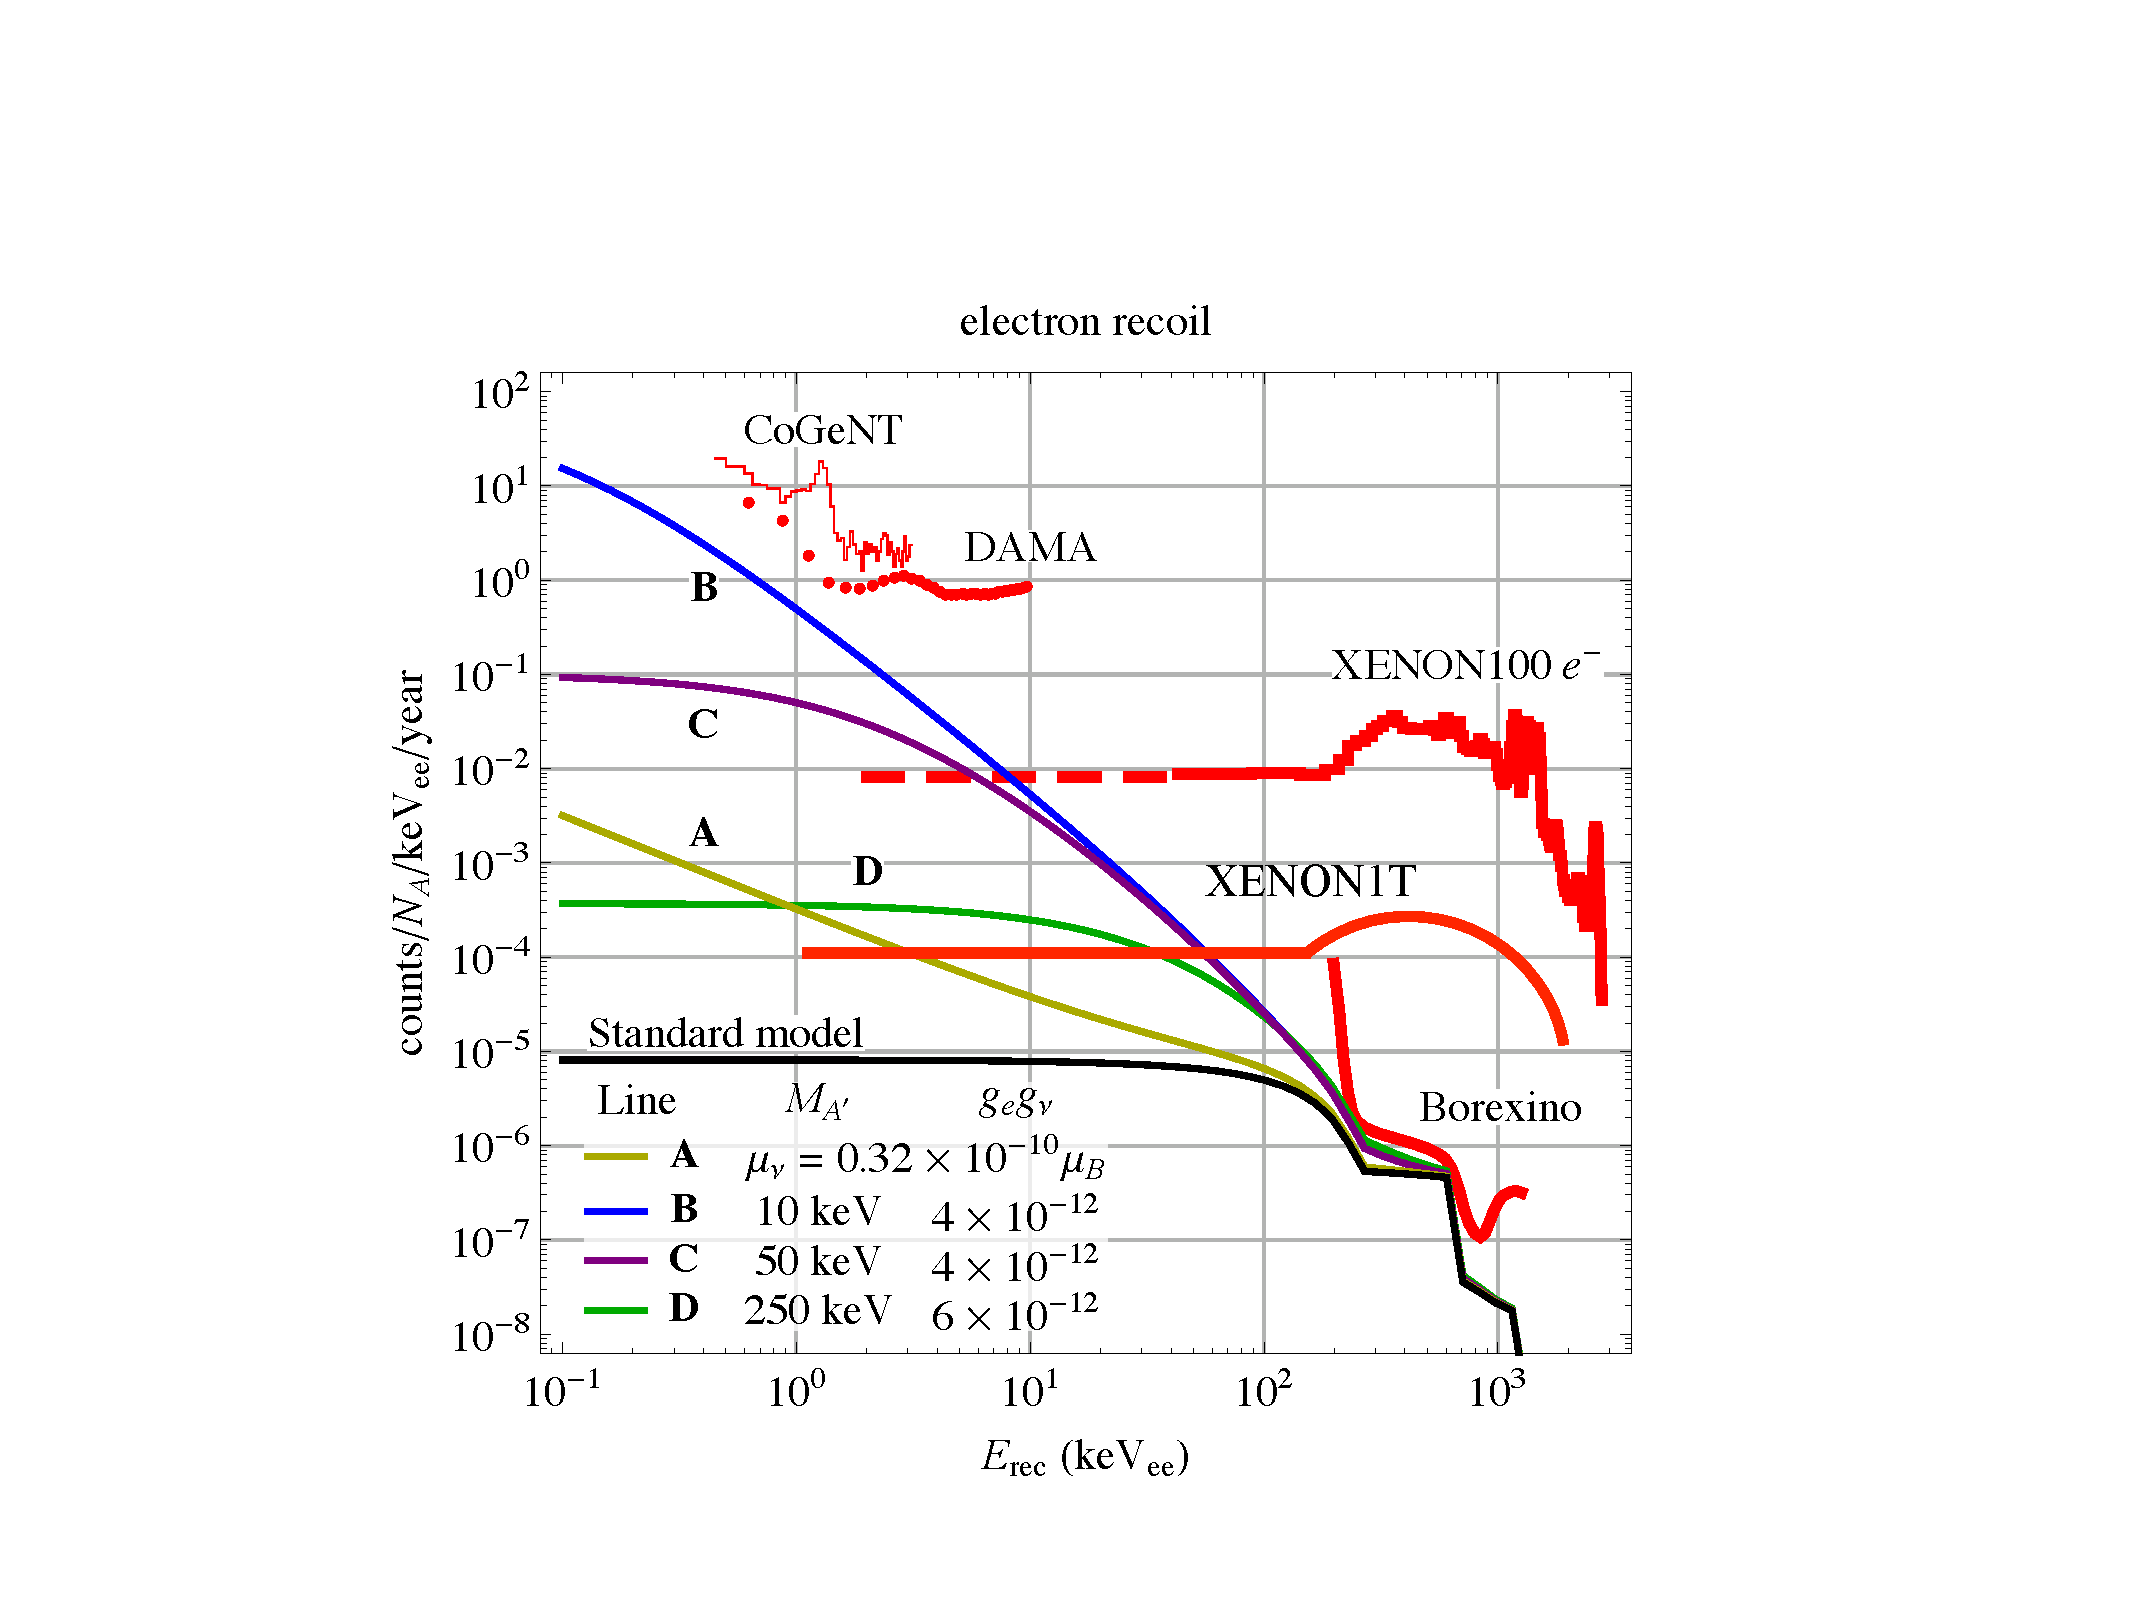
\includegraphics[width=0.47\textwidth]{fig_nu_in_dm.pdf}
\caption{\label{fig:NuInDM} Neutrinos can show up in dark matter experiments well above the neutrino fog. Shown in red are the electron recoil spectra in several experiments taken from~\cite{Harnik:2012ni}, with the recent spectrum measured by XENON1T indicated~\cite{Aprile:2017aty}. The spectrum expected from Standard Model solar neutrinos is in solid black. The solid colorful curves (A-D) are the solar neutrino spectra for several new physics models discussed in the text.}
\end{figure}

The next generation of experiments will have further sensitivity~\cite{Jeong:2021ivd,Babu:2021jnu}. In \autoref{fig:NuInDM} we show several spectra from new physics models which lead to an enhanced scattering rate at low energies. Curve~A shows the recoil spectrum in the case that the neutrino possesses a magnetic dipole moment around that which is allowed by current laboratory experiments (the limit by GEMMA~\cite{Beda:2012zz} is about 10\% lower). In this case the differential cross section is
\begin{equation}
\frac{\mathrm{d}\sigma}{\mathrm{d}E_r}= \mu_\nu^2 \alpha \left(\frac{1}{E_r}-\frac{1}{E_\nu}\right)
\end{equation}
where $\mu_\nu$ is the neutrino dipole moment and $E_r$ is the recoil energy of the electron. At high recoil energies, the dipole-induced scattering is lower than the Standard Model rate and in agreement with the Borexino rate. However, due to the $E_r^{-1}$ falloff, the rate is higher at low recoil energies. Already an analysis of XENON1T~\cite{Aprile:2020tmw} improves the limit in dipole moments to $<3\times 10^{-11}$ times a Bohr Magneton. The next-generation experiment will precisely measure the $pp$ solar neutrino spectrum at low energies and thus further improve this sensitivity.

One can also consider models with a faster falling spectrum. For example, curves B, C, and~D of \autoref{fig:NuInDM} are the spectra in a model with a new very light $B-L$ gauge boson which is mediating a new interaction between neutrinos and electrons. The cross section is
\begin{equation}
\frac{\mathrm{d}\sigma}{\mathrm{d}E_r}
%\propto \frac{1}{(q^2-m_{B-L}^2)^2}
=\frac{g_{B-L}^4 m_e}{4\pi (2m_e^2E_r^2 + m_{B-L}^2)^2}\,,
\end{equation}
where $m_{B-L}$ and $g_{B-L}$ are the mass and coupling. Here, we have dropped subleading terms in $E_r/E_\nu$ as well as interference with the SM process which is unimportant at most recoil energies. If the mass of the gauge boson is small, the cross section falls as $E_r^{-2}$. This behavior is due to the $1/(q^2-m_{B-L}^2)$ propagator in the amplitude, with $q^2=2m_e E_r$. Again it can be seen that a next-generation experiment will have significant sensitivity, well beyond that achieved by the Borexino experiment~\cite{Bellini:2011rx}, the GEMMA reactor experiment~\cite{Beda:2009kx}, or the XMASS experiment~\cite{Abe:2020nwr}. In fact, the discussion around the possible excess observed by XENON1T~\cite{Aprile:2020tmw} can already be used to place a constraint on $g_{B-L}<3.6\times 10^{-7}$ for mediators with mass $m_{B-L}<10\1{keV}$. This is already comparable with the constraint from GEMMA~\cite{Boehm:2020ltd}.  A next-generation liquid xenon experiment will be able to strengthen this bound.

It is interesting to consider a scenario in which the next generation of xenon experiments uncovers an excess above the solar neutrino fog. In this case we will immediately entertain both the possibility of dark matter and that of new neutrino physics, as evidenced by the list of papers discussing the excess observed by XENON1T~\cite{Aprile:2020tmw:refs}. Fortunately, this degeneracy can be disentangled with reactor neutrino experiments. To those that stand within 100~m of the core, nuclear reactors are a brighter source of neutrinos than the Sun. A low-threshold detector near a reactor, such as GEMMA~\cite{Beda:2009kx}, can thus place strong limits or distinguish whether an excess is coming from dark matter or neutrinos. \autoref{fig:NuMagMomSens} shows the current limits on the neutrino magnetic moment from both large underground detectors and reactor experiments, as well as the projected sensitivity for a next-generation liquid xenon detector with a 750 tonne-year exposure, complementary to dedicated experiments such as CONNIE~\cite{Aguilar-Arevalo:2016khx}. 

\begin{figure}[!htbp]
\centering
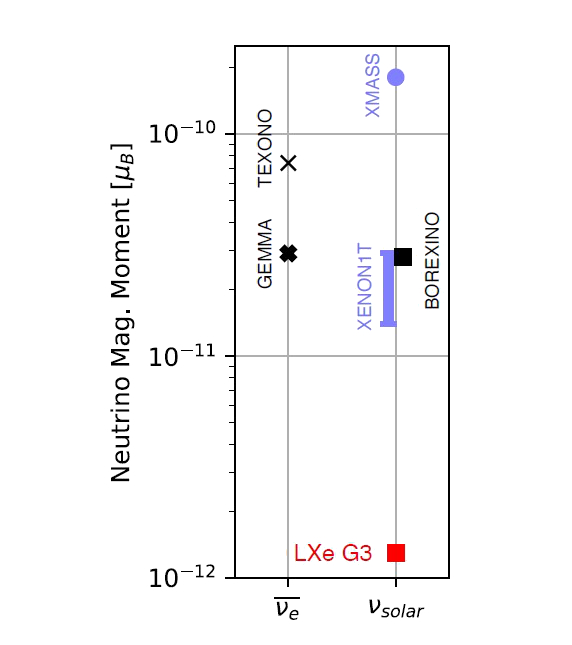
\includegraphics[width=0.4\textwidth]{fig_nu_magneticmoment_sensitivity.jpg}
\caption{\label{fig:NuMagMomSens} Projected neutrino magnetic moment sensitivity (red) along with current limits from reactor-based experiments (left markers) and experiments exposed to a solar flavor mixture (right markers). All the upper limits are reported at 90\% CL, except the XENON1T result, which shows the 10-90\% confidence interval~\cite{Abe:2020nwr,Borexino:2017fbd,Aprile:2020tmw}}
\end{figure}

In addition to the physics discussed in \autoref{sec:shortbaseline}, a mono-energetic neutrino source in combination with a large xenon detector could set very competitive sensitivities to neutrino magnetic dipole moments and sterile neutrino oscillation~\cite{Coloma:2014hka}. A 50-day run with a 3~MCi $^{51}Cr$ source produces 82~$\nu-e$ elastic scattering events in the XENON1T detector, which corresponds to 9.8 times better signal-to-noise ratio compared to using solar neutrinos~\cite{Coloma:2020voz}. The next-generation experiment discussed here could set much more stringent bounds on the neutrino magnetic moment, if combined with an electron capture source. 

\subsection{Fractionally Charged Particles}

The quantization of the electric charge has been one of the long-standing mysteries stemming from empirical observation. In principle, the Standard Model $U(1)$ allows arbitrarily small real-number charge, but so far, experiments indicate that there is a fundamental unit of electric charge of 1/3~e. This has sparked theoretical explanations including Dirac quantization~\cite{Dirac:1931kp} and provides one of the major motivations for a Grand Unification Theory (GUT)~\cite{Pati:1973uk,Georgi:1974sy}. The search for such fractionally charged or millicharged particles is a test of the paradigm of charge quantization~\cite{Dobroliubov:1989mr,Prinz:1998ua,Davidson:2000hf,Prinz:2001qz,Golowich:1986tj,Babu:1993yh,Gninenko:2006fi,CMS:2012xi,Agnese:2014vxh,Haas:2014dda,Ball:2016zrp,Alvis:2018yte,Magill:2018tbb,Kelly:2018brz,Berlin:2018bsc}. If such a particle was found, its small charge may or may not be the new electric charge unit, but in either case it will inevitably change our understanding of the current charge quantization built on quark charges, and contradict the predictions of certain GUTs.

One can consider the kinetic mixing between the SM $U(1)_Y$ and an additional gauge group $U(1)_D$, with additional matter particles $\xi$ charged under a dark $U(1)_D$. At low energies, one can effectively generate fractionally charged or millicharged particles in the limit when the dark $U(1)$ mediator (often called a dark photon, see \autoref{sec:dark_photon}) is massless. The level of kinetic mixing is usually $\sim 10^{-3}$ integrated from heavy fermion loops~\cite{Holdom:1985ag}, naturally giving small electric charges. One can also look for millicharged particles without massless gauge bosons in regimes where the dark photon is constrained~\cite{Kelly:2018brz}. A search for such a particle can be a test of GUTs and certain string compactification scenarios~\cite{Shiu:2013wxa}. Further, liquid xenon detectors are sensitive to the possible millicharge of solar neutrinos~\cite{Abe:2020nwr}.

\subsection{Nucleon Decay} 

In the Standard Model, the conservation of baryon number $B$ is an empirically observed symmetry. If $B$ were an exactly conserved quantum number, then protons, being the lightest baryons, would be stable. However, baryon number could be an approximate symmetry of Nature, and violated by small amounts, as predicted for example by many Grand Unified Theories. This could explain the observed matter-antimatter asymmetry of the universe~\cite{Babu:2013jba}. 

Several liquid xenon detectors, such as DAMA-LXe~\cite{Bernabei:2000xp,Bernabei:2006tw} and EXO-200~\cite{Albert:2017qto}, explored the possibility to investigate nucleon decay through so-called invisible decay modes, where the final states (neutrinos, or more exotic particles such as dark fermions) are not detected. One example for an invisible mode is $n \rightarrow \nu\nu\nu$, as proposed in~\cite{Mohapatra:2002ug}. Following such a decay, the daughter nuclei would be left in an excited state, and would emit a detectable signal, such as a $\gamma$-ray, once they de-excite. \autoref{tab_Xe} illustrates the various signatures for two xenon isotopes, $^{129}$Xe and $^{136}$Xe. These decays can be searched-for with a next-generation liquid xenon detector with unprecedented sensitivity.

\begin{table}[!htbp]
\footnotesize\centering
\begin{tabular}{lcll}
        & Invisible &          &  \\
        & decay     &          &  \\
Isotope & mode      & Daughter & Subsequent decays \\
\midrule
$^{129}$Xe & n   & $^{128}$Xe & stable                                                     \\
           & p   & $^{128}$I  & $^{128}$I $\rightarrow[Q = 2.217]{\text{$\beta^{-}$}}$ $^{128}$Xe \\
           &     &            & or $^{128}$I $\rightarrow[Q = 1.258]{\text{EC+$\beta^{+}$}}$ $^{128}$Te     \\
           & nn  & $^{127}$Xe & $^{127}$Xe $\rightarrow[Q = 0.664]{\text{EC}}$ $^{127}$I              \\
           & pn  & $^{127}$I  & stable                                                      \\
           & pp  & $^{127}$Te & $^{127}$Te $\rightarrow[Q = 0.694]{\text{$\beta^{-}$}}$ $^{127}$I      \\
\midrule
$^{136}$Xe & n   & $^{135}$Xe & $^{135}$Xe $\rightarrow[Q = 1.151]{\text{$\beta^{-}$}}$ $^{135}$Cs \\
           & p   & $^{135}$I  & $^{135}$I $\rightarrow[Q = 2.648]{\text{$\beta^{-}$}}$ $^{135}$Xe \\
           &     &            & \phantom{$^{135}$I} $\rightarrow[Q = 1.151]{\text{$\beta^{-}$}}$ $^{135}$Cs  \\
           & nn  & $^{134}$Xe & stable \\
           & np  & $^{134}$I  & $^{134}$I $\rightarrow[Q = 4.175]{\text{$\beta^{-}$}}$ $^{134}$Xe \\
           & pp  & $^{134}$Te & $^{134}$Te $\rightarrow[Q = 1.550]{\text{$\beta^{-}$}}$ $^{134}$I \\
           &     &            & \phantom{$^{134}$Te} $\rightarrow[Q = 4.175]{\text{$\beta^{-}$}}$ $^{134}$Xe  \\
           & nnn & $^{133}$Xe & $^{133}$Xe $\rightarrow[Q = 0.4274]{\text{$\beta^{-}$}}$ $^{133}$Cs \\
           & nnp & $^{133}$I  & $^{133}$I $\rightarrow[Q = 1.770]{\text{$\beta^{-}$}}$ $^{133}$Xe \\
           &     &            & \phantom{$^{133}$I} $\rightarrow[Q = 0.4274]{\text{$\beta^{-}$}}$ $^{133}$Cs \\
           & npp & $^{133}$Te & $^{133}$Te $\rightarrow[Q = 2.920]{\text{$\beta^{-}$}}$ $^{133}$I \\
           &     &            & \phantom{$^{133}$Te} $\rightarrow[Q = 1.770]{\text{$\beta^{-}$}}$ $^{133}$Xe \\
           &     &            & \phantom{$^{133}$Te} $\rightarrow[Q = 0.4274]{\text{$\beta^{-}$}}$ $^{133}$Cs \\
           & ppp & $^{133}$Sb & $^{133}$Sb $\rightarrow[Q = 4.003]{\text{$\beta^{-}$}}$ $^{133}$Te \\
           &     &            & \phantom{$^{133}$Sb} $\rightarrow[Q = 2.920]{\text{$\beta^{-}$}}$ $^{133}$I \\
           &     &            & \phantom{$^{133}$Sb} $\rightarrow[Q = 1.770]{\text{$\beta^{-}$}}$ $^{133}$Xe \\
           &     &            & \phantom{$^{133}$Sb} $\rightarrow[Q = 0.4274]{\text{$\beta^{-}$}}$ $^{133}$Cs \\
\end{tabular}
\caption{The daughter isotopes and their decay modes that follow the invisible mono- and di-nucleon decays of $^{129}$Xe and $^{136}$Xe as well as the tri-nucleon decays of $^{136}$Xe. This table is adapted after \cite{Bernabei:2000xp,Bernabei:2006tw}. The Q-values are reported in MeV.}
\label{tab_Xe}
\normalsize
\end{table}

\subsection{Short-Baseline Oscillations}\label{sec:shortbaseline}

Persistent anomalies in short baseline experiments, including LSND and MiniBooNE, are suggestive of an additional undiscovered neutrino mass eigenstate at the $\sim1\1{eV}$ mass scale~\cite{Abazajian:2017tcc}. However, there is significant tension between different experiments that has yet to be explained~\cite{Diaz:2019fwt}. Given the energy of $^{51}$Cr neutrinos, the oscillation pattern is expected to be within a meter-scale detector. This would make a next-generation liquid xenon TPCs well-suited to conclusively test the existence of sterile neutrinos~\cite{Coloma:2014hka}. In addition, such an experiment would be able to rule out portions of currently allowed parameter space, potentially resolving the existing tension if sterile neutrinos do not exist~\cite{Coloma:2014hka}.



